\section{Diagrama Entidad Relación}
\subsection{Diseño}
A continuación se observa el modelo completo que diseñamos como solución al problema planteado.

\begin{figure}[h!]
  \centering
  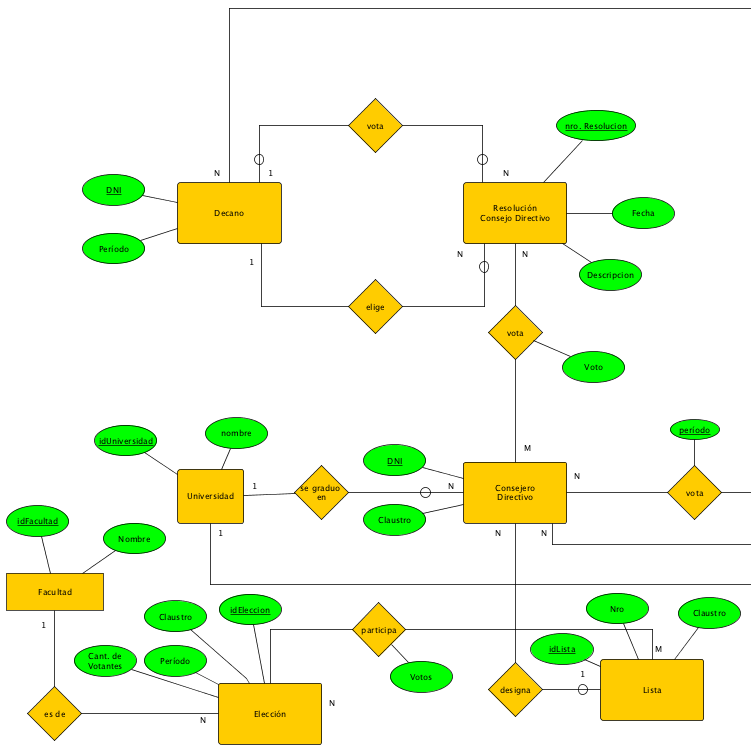
\includegraphics[width=1\textwidth]{./images/der1}
  \caption{Primera parte del Diagrama Entidad Relación}
  \label{fig:clases4}
\end{figure}

\begin{figure}[h!]
  \centering
  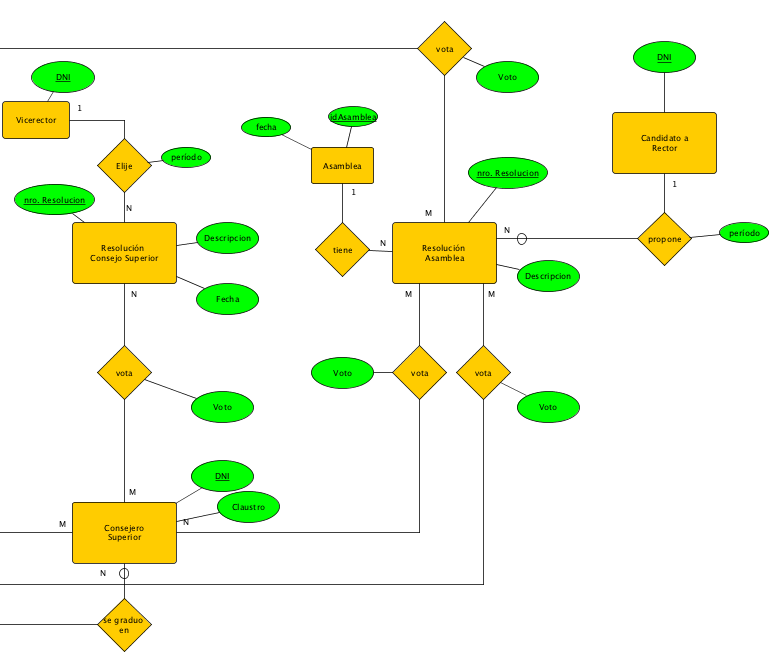
\includegraphics[width=1\textwidth]{./images/der2}
  \caption{Segunda parte del Diagrama Entidad Relación}
  \label{fig:clases4}
\end{figure}
\newpage
\subsection{Consideraciones}
Estas son algunas asunciones que hicimos con el fin de simplificar el modelo.

\begin{itemize}
\item  No es necesario tener la información de todo el padrón de cada claustro, ya que la votación de consejeros directivos es secreta.
\item Al no modelar los integrantes de cada claustro no modelamos las condiciones que deben cumplir los candidatos a los diferentes cargos. Asumimos que las personas que estan en cada una de esas tablas cumplen las condiciones. Esto es:
	\begin{itemize}
    \item Pueden ser candidatos por el claustro de profesores los profesores titulares plenarios, titulares asociados, profesores consultos y eméritos de cualquier Facultad de la UBA.
    \item Pueden ser candidatos por el claustro de graduados quienes hayan obtenido su diploma por la UBA (siempre y cuando no sean profesores) o los graduados de otras universidades nacionales con iguales títulos si acreditan actividad profesional de al menos dos años en la UBA.
    \item Pueden ser candidatos por el claustro de estudiantes cualquier alumno regular de una carrera que tengan al menos un año de antiguedad en la inscripción.
    \item Para ser rector hace falta ser ciudadano argentino, tener 30 años o más y ser o haber sido profesor de alguna Universidad Nacional.
    \end{itemize}
\item Las resoluciones rechazadas también son registradas: para cada par resolución/consejero, el atributo de la relación ''vota'' (llamado ''voto'') indica si el mismo fue positivo o negativo. Contabilizando los votos positivos sobre el total se puede saber si la resolución fue aprobada o no.
\item Por el mismo motivo, no modelamos explícitamente cuando un candidato a decano/rector es efectivamente elegido, sino que esta informacion se deduce de la cantidad de votos que recibió cada candidato. Esto es porque las elecciones se realizan por medio de resoluciones: cada consejero vota una resolución que promueve a su candidato como decano/rector. De esas resoluciones, la que resulta finalmente aprobada 'elige'' al decano/rector ganador. De esta manera podemos saber a qué candidato vota cada consejero, y también detectar empates o falta de quórum (si ninguna resolución de cierta fecha terminó eligiendo un candidato).
\end{itemize}

\subsection{Aclaraciones}
Estas son algunas aclaraciones a tener en cuenta sobre cosas que podrían no quedar claras en el DER.
\begin{itemize}
\item En nuestro afán de evitar la redundancia, podría parecer que hay información faltante (por ejemplo, de qué facultad es cierto Consejero Directivo), sin embargo nos preocupamos mucho por que toda la información necesaria sea accesible de algún modo (el Consejero es designado por una Lista que participa en una Elección que pertenece a una Facultad).
\item No incluimos en el modelo la totalidad de atributos de las entidades que podrían resultar interesantes, porque consideramos que esa información puede cambiar rápidamente y el enunciado no especifica cuáles son. Naturalmente entendemos que quien opere la base va a querer guardar el apellido de los candidatos, la dirección de las Facultades, el texto completo de las resoluciones, etc., pero por economía de espacio y para no sobre-especificar decidimos dejar la elección de los atributos a una etapa posterior. Sí incluimos, como puede observarse, todos los atributos necesarios para obtener la información necesaria para resolver las consultas especificadas.
\end{itemize}

\subsection{Restricciones}
Para que el modelo cumpla con lo estipulado en el estatuto, se deben tener en cuenta las siguientes restricciones extras:

\begin{itemize}
\item Una misma lista no puede estar en dos elecciones de distintas facultades.
\item Todas las resoluciones de Consejo Directivo son votadas por consejeros de la misma facultad.
\item Los consejeros directivos solo votan consejeros superiores de su propio claustro.
\item 'M' es 5 en la relación de votación de Consejero Directivo y Consejero Superior
\item Las resoluciones de Consejo Directivo son votadas por 4 Consejeros estudiantiles, 4 graduados y 8 profesores, correspondientes a la facultad y período de la resolución.
\item La composición del Consejo Directivo cumple lo especificado en el estatuto (por ejemplo para estudiantes, 3 para la mayoría y 1 para la primer minoría si llega al 20\% de los votos).
\item Las resoluciones que forman parte de la relación ''vota'' con un decano/rector son las que proponen a un candidato como decano/rector. Las que además forman parte de la relación ''elige'' son las ganadoras de esa elección.
\item Ningún consejero puede ser representante por dos claustros en el mismo período.
\end{itemize}

\section{Modelo Relacional}
Este es el MR correspondiente a DER presentado anteriormente. En él se pueden ver las distintas tablas necesarias para realizar la implementación.


\noindent \textbf{Decano}(\underline{DNI}, Periodo) \\
\textbf{ResolucionConsejoDirectivo}(\underline{nroResolucion}, Fecha, \dashuline{idDecanoQueVota}, \\\dashuline{idDecanoElegido})\\
\textbf{ResolucionConsejoSuperior}(\underline{nroResolucion}, Fecha)\\
\textbf{Asamblea}(\underline{idAsamblea}, fecha)\\
\textbf{ResolucionAsamblea}(\underline{nroResolucion}, \dashuline{idAsamblea, idCandidatoRector, idCandidatoVicerrector})\\
\textbf{CandidatoARector}(\underline{DNI}, periodo)\\
\textbf{Universidad}(\underline{idUniversidad}, nombre)\\
\textbf{ConsejeroDirectivo}(\underline{DNI}, Claustro, \dashuline{idUniversidad, idLista})\\
\textbf{ConsejeroSuperior}(\underline{DNI}, Claustro, \dashuline{idUniversidad})\\
\textbf{Lista}(\underline{idLista}, Nro, Claustro)\\
\textbf{Facultad}(\underline{idFacultad}, Nombre)\\
\textbf{Eleccion}(\underline{idEleccion}, Periodo, CantDeVotantes, \dashuline{idFacultad})\\
\textbf{CandidatoAVicerrector}(\underline{DNI})\\
\textbf{VotaDecanoAsamblea}(\underline{idDecano, nroResolucion}, voto)\\
\textbf{VotaSuperiorAsamblea}(\underline{DNI}, voto)\\
\textbf{VotaDirectivoAsamblea}(\underline{DNI}, voto)\\
\textbf{VotaResolucionDirectivo}(\underline{DNI, nroResolucion}, voto)\\
\textbf{VotaResolucionSuperior}(\underline{DNI, nroResolucion}, voto)\\
\textbf{VotaDirectivoSuperior}(\underline{DNI\_Directivo, DNI\_Superior, periodo})\\
\textbf{Participa}(\underline{idLista, idEleccion})\\


\section{Consultas}

En esta sección vamos a explicar en castellano cómo se pueden resolver las consultas pedidas en el enunciado.

\begin{itemize}
\item \textbf{La cantidad de elecciones de Rector que requirieron al menos 3 sesiones de votación para llegar a un resultado satisfactorio}

Nuestro modelo considera la tabla de candidatos a Rector donde se registra los distintos candidatos. Cada uno de estos candidatos está relacionado con su resolución de asamblea correspondiente, considerando el período al cual se postula. Al contabilizar los votos de cada uno de los asambleístas se logra identificar aquellos cuya cantidad de votos no alcanza para asumir.
Al tener como atributo relacional el período podemos considerar aquellos períodos para los cuales fue necesario variadas instancias de votación: si resoluciones de asambleas distintas proponen un rector para el mismo período quiere decir que fueron necesarias varias elecciones para elegirlo.

\item \textbf{Los nombres de las 5 personas con mayor cantidad de participaciones en Asambleas Universitarias}

Al tener el DNI como atributo de los distintos cargos nominales de los órganos de cogobierno es sencillo buscar aquellas personas que fueron parte de asambleas universitarias, no importa cual haya sido su cargo, viendo las resoluciones de las asambleas y votaciones en las cuales participaron.

\item \textbf{Porcentaje  histórico  de  representantes  del  Claustro  de  Graduados  de  la UBA que se graduaron en otra universidad nacional}

Para esto, guardamos para aquellos consejeros (Directivos o Superiores) que sean graduados la información de en qué Universidad se graduaron. De este modo, podemos calcular el porcentaje de graduados que se graduaron en otra universidad nacional. Se deberá tener en cuenta que sean personas distintas (DNI distinto) ya que una persona puede ser Consejero varios años y en varios cuerpos (por ejemplo ser primero Directivo y luego Superior).

\item \textbf{Resolución de algunas de las restricciones del enunciado utilizando triggers}
Podemos hacer que el motor cree automáticamente las relaciones ''elige'' cuando un candidato a Decano/Rector tiene suficientes votos positivos en la Resolución correspondiente a su designación. Solo hace falta implementar las reglas para la elección de cada uno de ellos:
  \begin{itemize}
  \item El Decano requiere por lo menos 9 de 16 votos.
  \item El Rector requiere la mitad más uno de los votos, salvo que sea la tercera vez que se reúne la asamblea para este período, en cuyo caso solo le hace falta superar a todos los demás candidatos.
  \end{itemize}
\end{itemize}





